\chapter{突触的形成和消除} \label{chap:chap48}


到目前为止,我们已经研究了哺乳动物神经系统发育的三个阶段:
神经管的形成和模式化、神经元和神经胶质细胞的生成和分化,以及轴突的生长和引导。
在大脑发挥功能之前必须进行一个额外的步骤:突触的形成。
只有当突触形成并发挥作用时,大脑才能处理信息。


三个关键过程驱动突触形成。
首先,轴突在许多\textit{突触后电位}伙伴中做出选择。
通过仅在特定目标细胞上形成突触连接,神经元组装可以处理信息的功能回路。
在许多情况下,突触甚至在突触后细胞的特定位置形成;
一些类型的轴突在树突上形成突触,另一些在细胞体上形成突触,还有一些在轴突或神经末梢上形成突触。
尽管细胞和亚细胞特异性在整个大脑中都很明显,但突触形成的一般特征可以用几个经过充分研究的例子来说明。


其次,在细胞-细胞接触形成后,轴突接触靶细胞的部分分化为突触前神经末梢,轴突接触的靶细胞区域分化为专门的突触后装置。
突触前和突触后分化的精确协调取决于轴突与其靶细胞之间的相互作用。
我们对这些相互作用的了解大部分来自对神经肌肉接头的研究,神经肌肉接头是运动神经元和骨骼肌纤维之间的突触。
这种突触的简单性使其成为探索化学突触的结构和电生理学原理的有利系统(第~\ref{chap:chap12}~章),这种简单性也有助于分析发育中的突触。
我们将使用神经肌肉突触来说明突触发育的关键特征,然后应用来自该外周突触的见解来检查大脑中形成的突触。


最后,一旦形成,突触就会成熟,通常会进行重大重排。
重排的一个显著方面是,随着一些突触的生长和强化,许多其他突触被消除。
与神经元细胞死亡(第~\ref{chap:chap46}~章)一样,突触消除乍一看是神经发育过程中一个令人费解且看似浪费的步骤。
然而,越来越清楚的是,它在完善连接的初始模式方面发挥着关键作用。
我们将讨论突触在神经肌肉接头处重排的主要特征,它已被深入研究,以及在神经元之间的突触处,它也很突出。


在组装神经系统的一系列事件中,突触形成处于一个有趣的交叉点。
这个过程的初始步骤似乎在很大程度上是由分子程序“固定”的。
然而,一旦突触形成,神经系统就开始发挥作用,神经回路的激活在随后的发育中起着至关重要的作用。
事实上,神经系统的信息处理能力通过它的使用而得到完善,在出生后早期最为显著,但也会进入成年期。
从这个意义上说,神经系统在整个生命过程中不断发育。
我们将在描述突触形成和重排时考虑分子程序和神经激活的相互作用。
这个讨论将是第~\ref{chap:chap49}~章的一个有用的前奏,在该章中我们将讨论基因和环境(先天和后天)如何相互作用以在出生后早期定制神经系统。



\section{神经元识别特定的突触目标}

一旦轴突到达指定的目标区域,它们就必须从许多容易到达的潜在目标中选择合适的突触伙伴。
尽管突触形成在细胞和亚细胞水平上都是一个高度选择性的过程,但很少有赋予突触特异性的分子被鉴定出来。


当交织在一起的轴突选择目标细胞的子集时,突触连接的特异性尤为明显。
在这些情况下,可以区分轴突引导和选择性突触形成。
这种特异性的第一份报告出现在100多年前,当时\textit{兰列}在研究自主神经系统时提出了化学特异性假说的第一个版本(见第~\ref{chap:chap46}~章)。
\textit{兰列}观察到自主神经节前神经元是在脊髓不同的头尾水平产生的。
它们的轴突一起进入交感神经节,但与支配不同目标的不同突触后神经元形成突触。
如图~\ref{fig:48_1}A~所示,以行为分析为指导,\textit{兰列}推断位于脊髓延髓头端的神经节前神经元的轴突在神经节神经元上形成突触,神经节神经元将其轴突投射到相对延髓的目标(例如眼睛),而来自脊髓更多尾部区域的神经元投射到尾部目标(例如耳朵)的神经节神经元上形成突触。
然后他表明,如图~\ref{fig:48_1}B~所示,在节前轴突被切断并允许再生后,类似的模式被重新建立,这使他推测某种分子识别起了作用。


\begin{figure}[htbp]
	\centering
	\includegraphics[width=1.0\linewidth]{chap48/fig_48_1}
	\caption{节前运动神经元与其交感神经元目标重新生成选择性连接。
		A. 节前运动神经元起源于胸脊髓的不同水平。
		位于嘴侧的胸神经元产生的轴突支配颈上神经节神经元,这些神经元投射到嘴侧目标,包括内在眼部肌肉。
		起源于胸髓尾侧水平的神经元的轴突支配神经节神经元,这些神经元将轴突投射到更尾侧的目标,如耳朵的血管。
		这两类神经节神经元在神经节中混合在一起,这使\textit{兰列}提出,来自不同胸部水平的神经节前轴突选择性地与终止于特定外周目标的神经节神经元形成突触。
		B. 成年神经损伤后,在神经再支配过程中会形成类似的节段特异性连接模式,这支持了突触形成具有选择性的观点\cite{njaa1977specific}。}
	\label{fig:48_1}
\end{figure}


电生理学研究后来证实了\textit{兰列}关于这些神经节突触连接特异性的直觉。
此外,这种选择性在神经支配的早期阶段是显而易见的,即使特定类型的突触后神经元散布在神经节内。
成年后神经损伤后选择性的重新建立表明,特异性不会通过胚胎时间或神经元定位的特殊性出现。



\subsection{识别分子促进视觉系统中选择性突触的形成}

为了更详细地说明目标特异性的概念,我们将首先考虑视网膜神经节细胞。
这些神经元的反应特性不同:一些神经节神经元对光照强度的增加有反应(给光细胞),其他神经元对光照强度降低(撤光细胞)有反应,其他神经元对移动物体有反应,还有一些对特定颜色的光有反应。
所有神经节细胞的轴突都穿过视神经,形成从视网膜到大脑的并行轴突通路。


每一类神经节细胞的反应特性取决于它们从无长突和双极中间神经元接收的突触输入,这些中间神经元又从光敏光受体接收突触。
从双极细胞和无长突细胞到神经节细胞树突的所有突触都发生在视网膜的一个狭窄区域,称为\textit{内网层}。
因此,轴突和树突有一项艰巨的任务,即在一大群不合适的旁观者中识别出它们正确的伙伴。


\textit{内网层}中突触匹配的一个重要贡献是它分成子层。
每种无长突细胞和双极细胞类型的过程,以及每种功能不同的神经节细胞类型的树突、分支和突触仅在大约 10 个子层中的一个或几个子层中。
例如,\textit{给光细胞}和\textit{撤光细胞}的树突分别限制在\textit{内网层}和\textit{外网层},因此接收来自不同中间神经元的突触;
如图~\ref{fig:48_2}~所示,特定类型的\textit{给光细胞}和\textit{撤光细胞}在这些区域内具有更窄的限制。
这种层特异性的突触前和突触后进程的分支,限制了它们容易接触到的突触伙伴的选择。
在大脑和脊髓的许多其他区域也发现了类似的层板特异性连接。
例如,在大脑皮层中,不同的轴突群将它们的树突状结构和突触限制在六个主要层中的一两个。


\begin{figure}[htbp]
	\centering
	\includegraphics[width=1.0\linewidth]{chap48/fig_48_2}
	\caption{视网膜神经节神经元形成层特异性突触。
		A. 视网膜神经节神经元的树突接收来自\textit{内网层}中的视网膜中间神经元(无长突细胞和双极细胞)过程的输入,该层被细分为至少 10 个子层。
		中间神经元和神经节细胞的特定子集通常仅在一层中分支和形成突触。
		这些层特异性连接决定了哪些视觉刺激的方面(它们的开始或结束)激活每种类型的视网膜神经节细胞。
		右侧显示了\textit{撤光}和给光视网膜神经节细胞的反应。
		B. 免疫球蛋白超家族粘附分子(Sdk1、Sdk2、Dscam 和 DscamL)在发育中的鸡胚中由无长突和视网膜神经节神经元的不同亚群表达。
		表达这四种蛋白质之一的无长突神经元与表达相同蛋白质的视网膜神经节细胞形成突触。
		操纵 Sdk 或 Dscam 表达式会改变这些层特异性分支的模式。}
	\label{fig:48_2}
\end{figure}


% Laminar specificity does not, however, completely
然而,层流特异性并不能完全解释视网膜的连接方式。
由于视网膜细胞类型的数量(目前在小鼠中估计约为 130 个)大大超过丛状亚层的数量,因此许多细胞类型的突起在每个亚层内分叉。
解剖学和生理学研究表明,即使在单个子层内,连通性也是特定的。
此外,连接模式似乎在很大程度上(尽管不完全)是“硬连线”的,发生在\textit{视觉经验}有机会影响回路之前。
因此,必须存在将轴突和树突限制在特定亚层的分子,以及区分亚层内突触伙伴的分子。


% One clue to the basis of both laminar
视网膜中层状和层内突触特异性基础的一条线索来自于这样一个发现:特定类型的中间神经元和神经节神经元表达不同类别的免疫球蛋白和钙粘蛋白家族的识别分子(第~\ref{chap:chap47}~章)。
因此,如图~\ref{fig:48_2}B~所示,表达特定识别分子的细胞过程仅限于一个或几个丛状亚层。
许多这些蛋白质促进嗜同性相互作用;
也就是说,它们与其他细胞表面的相同蛋白质结合。
现在已经在鸡和小鼠视网膜中评估了几种识别分子的作用,方法是在发育过程中去除它们,或者将它们植入通常不表达它们的神经元中。
这些所谓的“功能丧失”和“功能获得”实验的结果暗示存在一种复杂的识别分子编码,可促进目标区域内的特定连接。
例如,在小鼠中,两个钙粘蛋白将双极中间神经元引导至适当的亚层,而 Sidekick 2 免疫球蛋白超家族的一个成员,是中间神经元在一个特定亚层中具有树突的神经节细胞中进行选择所必需的。



\subsection{感觉受体促进嗅觉神经元的靶向}

嗅觉系统中有一种不同类型的特异性。
鼻上皮细胞中的每个嗅觉感觉神经元只表达大约 1 千种气味受体中的一种。


如图~\ref{fig:48_3}A~所示,表达同一种受体的神经元随机分布在大部分上皮细胞中,但它们的所有轴突都聚集在嗅球中少数目标神经元的树突上,形成富含突触的小球。
如图~\ref{fig:48_3}B~所示,当单个嗅觉受体被删除时,通常表达受体的轴突到达嗅球但不能汇聚到特定的肾小球或终止于适当的突触后细胞。
相反,如图~\ref{fig:48_3}C~所示,当神经元被迫表达不同的气味受体时,它们的轴突在嗅球内的不同位置形成小球。


\begin{figure}[htbp]
	\centering
	\includegraphics[width=0.69\linewidth]{chap48/fig_48_3}
	\caption{气味受体影响感觉轴突靶向嗅球中离散的球状体\cite{sanes2009many}。
		A. 每个嗅觉受体神经元表达大约 1 千种可能的气味受体中的一种。
		表达相同受体的神经元稀疏地分布在整个鼻子的嗅觉上皮细胞中。
		这些神经元的轴突与嗅球中单个小球中的目标神经元形成突触。
		B. 在气味受体基因被删除的小鼠突变体中,本应表达该基因的感觉神经元将其轴突发送到其他小球,部分原因是这些神经元现在表达了其他受体。
		C. 当一组感觉神经元中的一个气味受体基因取代另一个时,它们的轴突投射不正常。}
	\label{fig:48_3}
\end{figure}


总之,这些实验表明,嗅觉受体不仅决定了神经元对特定气味的反应,而且还帮助轴突在目标神经元上形成适当的突触。
最初,人们怀疑特定的嗅觉受体不仅可以作为气味探测器,还可以作为识别分子。
最近的研究为不同的机制提供了证据:
由嗅觉受体激活产生的第二信使影响识别分子的表达,这些识别分子将嗅觉轴突与嗅球中的适当目标相匹配。


匹配分两步进行。
首先,嗅觉受体刺激第二信使环磷酸腺苷形成的能力存在内在差异,导致胚胎中引导分子的差异表达,从而产生沿前后轴的嗅觉神经元和嗅球目标的粗略匹配。
其次,4 组嗅觉感觉神经元选择性表达识别分子,将它们定位到沿嗅球背腹轴的相应区域。


因此,如图~\ref{fig:48_4}A~所示,分子识别的早期阶段通过与激活无关的机制生成了一个粗略的鼻脑连通性映射。
然后,在出生后,气味受体被气味激活,并且由于细胞内信号的发育变化,这种激活导致第二组识别分子的诱导。
如图~\ref{fig:48_4}B~所示,这些分子导致轴突会聚到球状体上,从而通过激活依赖机制改进投射。
通过粘附和排斥相互作用,轴突首先分离到特定区域,然后分离到特定球状体。


\begin{figure}[htbp]
	\centering
	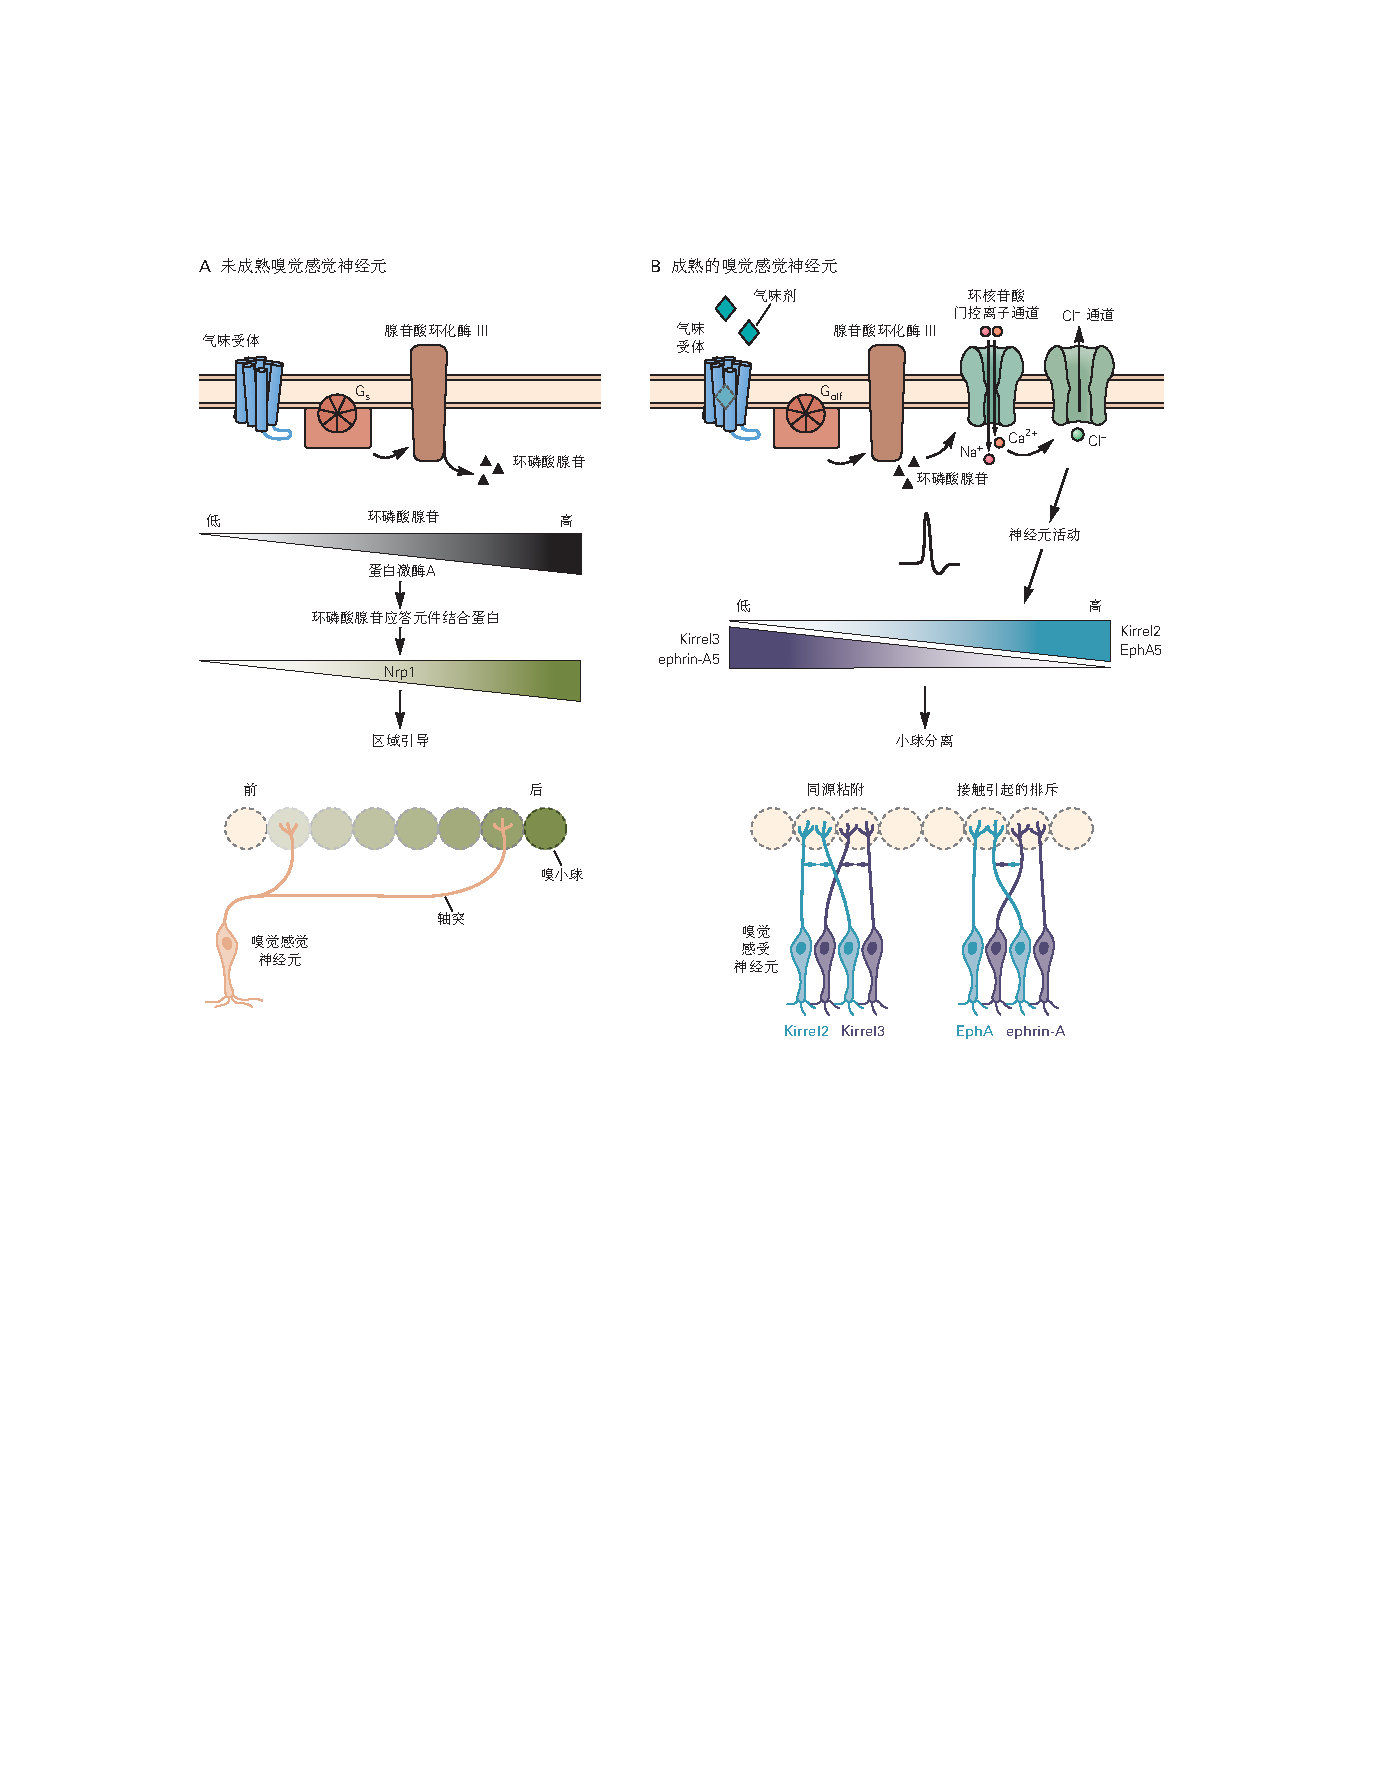
\includegraphics[width=1.0\linewidth]{chap48/fig_48_4}
	\caption{气味受体通过控制引导和识别分子的表达来促进嗅球中的特定连接。
		嗅觉感觉神经元中嗅觉受体的激活导致\textit{腺苷酸环化酶}的激活和第二信使\textit{环磷酸腺苷}产生。
		A. 出生前,在嗅觉发生之前,受体是自发激活的。
		不同类型的受体表现出不同程度的自发激活,因此产生不同水平的\textit{环磷酸腺苷},进而诱导不同的、分级水平的轴突引导分子,如\textit{神经轴突指导分子}和\textit{信号素}。
		这些引导分子介导轴突之间的相互作用,引导它们到达嗅球的适当区域。
		B. 出生后,嗅觉受体被气味分子激活。
		这种嗅觉激活还在每种类型的气味受体神经元中产生不同水平的 \textit{环磷酸腺苷},但现在第二信使通过离子通道起作用以诱导新的引导分子组,例如 kirrels 和肝配蛋白。
		这些分子介导相互作用,将轴突末端分离到球状体中。
		因此,受体激活的连续阶段,首先是自发的,其次是由气味引起的,共同作用以将不同类型的嗅觉感觉轴突映射到不同的球状体上。}
	\label{fig:48_4}
\end{figure}



\subsection{不同的突触输入被定向到突触后细胞的离散域}


神经末梢不仅可以区分候选目标,还可以终止于目标神经元的特定部分。
例如,在大脑皮层和海马体中,到达分层结构的轴突通常将它们的末端限制在一层,即使突触后细胞的树突树穿过许多层也是如此。
在小脑中,不同类型神经元的轴突终止于浦肯野神经元的不同区域。
如图~\ref{fig:48_5}~所示,\textit{颗粒细胞的轴突}接触远端树突棘,\textit{攀援纤维的轴突}接触近端树突轴,\textit{篮状细胞的轴突}接触轴丘和起始段。


\begin{figure}[htbp]
	\centering
	\includegraphics[width=0.84\linewidth]{chap48/fig_48_5}
	\caption{小脑中抑制性中间神经元的轴突终止于小脑浦肯野细胞的一个特定区域。
		许多神经元在小脑浦肯野神经元形成突触,每个神经元在浦肯野细胞上选择一个不同的区域。
		抑制性\textit{篮状细胞的轴突}大部分在轴丘和初始段形成突触。
		篮状细胞通过识别\textit{神经束蛋白}来选择这些结构域,神经束蛋白是一种细胞表面免疫球蛋白超家族粘附分子,通过\textit{锚定蛋白 G} 锚定在轴突的初始段。
		当神经束蛋白的定位受到干扰时,篮状细胞轴突无法将突触形成限制在初始段\cite{huang2006subcellular}。}
	\label{fig:48_5}
\end{figure}


这种特异性可能依赖于突触后细胞表面的分子信号。
对于小脑的浦肯野神经元,\textit{神经束蛋白}就是这样的一个信号,它是免疫球蛋白超家族的一种粘附分子。
\textit{神经束蛋白}在轴突起始段上以高水平存在,从而引导\textit{篮状细胞}在该轴突区域选择性地形成轴突。
因此,粘附分子也可以作为神经元特定区域的识别分子。
由于单个神经元可以与多类突触前细胞和突触后细胞形成突触,因此每个神经元亚型必须表达多种突触识别分子。



\subsection{神经激活增强突触特异性}


到目前为止,我们已经强调了识别分子在突触初始形成中的作用。
然而,一旦突触形成,回路中的神经激活在完善突触模式中起着关键作用。
例如,如上所述,嗅觉神经元到嗅球的引导包括初始激活独立粗映射,然后是激活依赖阶段,其中投射被细化。


在视觉系统中已经详细研究了类似的双相模式。
如图~\ref{fig:48_6}~所示,\textit{视网膜神经节细胞}投射到\textit{视顶盖}(上丘),其中肝配蛋白和 Eph 激酶之间的相互作用导致在顶盖表面形成视网膜轴突的粗略\textit{视网膜映射}(第~\ref{chap:chap47} 章)。
然后,激活依赖过程塑造了视网膜神经节细胞的轴突树突。
轴突最初形成广泛而分散的树突,随着时间推移,这些树突逐渐变得更密集但更集中,使顶盖映射更加清晰。
当突触的激活被阻断时,这种细化就会受到抑制。
这种依赖于激活改进的分子机制在很大程度上是未知的。
与嗅觉系统一样,一个有吸引力的想法是神经元激活的水平和模式调节识别分子的表达。


\begin{figure}[htbp]
	\centering
	\includegraphics[width=1.0\linewidth]{chap48/fig_48_6}
	\caption{电激活改进了\textit{视网膜神经节细胞}突触连接的特异性。
		一些视网膜神经节细胞最初形成树突状树突,仅限于视网膜\textit{内网层}的特定亚层,而其他细胞最初形成弥漫性树突,后来被修剪以形成大的特定模式。
		同样,视网膜神经节细胞的轴突树突最初支配\textit{上丘}中目标区域的大片区域。
		然后细化这个广泛的轴突树突被细化,以便将许多分支集中在一个小区域。
		消除视网膜神经节细胞中的电激活会减少树突和轴突树突的重塑。}
	\label{fig:48_6}
\end{figure}


这些来自嗅觉和视觉系统的例子说明了一个广泛存在的现象:
分子线索最初控制着突触的特异性,但一旦回路开始发挥作用,特异性就会通过神经激活而增强。
在视觉系统中,细化涉及突触的丢失。
我们将在本章末回到突触消除这个过程,并在下一章考虑它对行为的影响。


在一些情况下,神经激活通过将不合适的目标变成合适的目标,以不同的方式促进特异性。
这种机制在骨骼肌中得到了最清楚的证明,其中哺乳动物的肌肉纤维可以根据其收缩特性分为几类(第~\ref{chap:chap31}~章)。
特定类型的肌纤维表达主要收缩蛋白(如肌球蛋白和肌钙蛋白)独特亚型的基因。


很少有肌肉完全由单一类型的纤维组成;
大多数都有各种类型的纤维。
然而,如图~\ref{fig:48_7}A~所示,单个运动轴突的分支支配单一类型的肌肉纤维,即使在不同类型的纤维混合的“混合”肌肉中也是如此。
这种模式意味着显著程度的突触特异性。
然而,匹配并不总是通过运动轴突识别适当类型的肌纤维来实现。
运动轴突还可以将目标肌肉纤维转换为适当的类型。
当肌肉在出生时失去神经支配,在其纤维特性固定之前,通常支配慢速肌肉的神经可以重新定向以支配注定要变快的肌肉,反之亦然。
如图~\ref{fig:48_7}B、C~所示,在这些条件下,肌肉的收缩特性在运动神经的放电特性强加的方向上发生部分变化。


\begin{figure}[htbp]
	\centering
	\includegraphics[width=1.0\linewidth]{chap48/fig_48_7}
	\caption{运动神经元激活的模式可以改变骨骼肌细胞的生化特性和功能特性。
		A. 肌肉纤维具有特征性的代谢、分子和电学特性,可将它们识别为“慢速”(强直)或“快速”(阶段性)类型。
		右侧的显微照片显示了肌球蛋白\textit{三磷酸腺苷酶}的组织化学染色的肌肉组织切片。
		中间的草图显示了肌肉的一部分,其中运动神经元(绿色和棕色)在单一类型的肌肉纤维上形成突触。
		B. 连接快肌和慢肌纤维的运动神经元(快运动神经元和慢运动神经元)表现出不同的电激活模式:
		稳定的低频(强直)放电用于慢纤维和间歇性高频突发(相位)用于快纤维。
		C. 交叉神经支配实验表明,运动神经元的某些特性有助于确定肌纤维是快还是慢。
		交叉神经支配是通过手术将快速轴突重新路由到慢速肌肉来实现的,反之亦然。
		尽管运动神经元的特性变化不大,但肌肉的特性却发生了深刻的变化。
		例如,快速运动神经元在慢肌中诱发快速特性\cite{salmons1976significance}。
		D. 快神经和慢神经对肌肉的神经支配的影响部分是由它们不同的激活模式介导的。
		以慢速强直模式刺激快肌可将肌肉转变为慢速型。
		相反,对慢速肌肉的快速相位刺激可以将其转化为更快的类型。}
	\label{fig:48_7}
\end{figure}


快速运动神经元和慢速运动神经元中不同的神经激活模式是肌肉特性转换的原因。
最引人注目的是,如图~\ref{fig:48_7}D~所示,以通常由慢神经或快神经诱发的模式对肌肉进行直接电刺激会导致几乎与交叉神经支配一样的显著变化。
尽管在神经肌肉接头处观察到的基于激活的类型转换不太可能是中枢神经系统突触特异性的主要贡献者,但中枢轴突很可能会改变其突触目标的特性,从而促进神经元亚型的多样化,并改进由识别分子施加的连接。



\section{神经肌肉接头处揭示了突触分化的原理}

神经肌肉接头包括三种类型的细胞:
运动神经元、肌纤维和\textit{施旺细胞}。
所有三种类型在突触区域都高度分化。


当运动轴突在第~\ref{chap:chap47}~章中描述的多种因素的引导下,到达发育中的骨骼肌并接近未成熟的肌纤维时,突触形成过程就开始了。
接触发生后,突触分化过程便开始了。
当生长锥开始转变为神经末梢时,与神经末梢相对的肌肉表面部分开始获得其自身的特化。
随着发育的进行,突触成分被添加,突触分化的结构迹象在突触前和突触后细胞以及突触间隙中变得明显。
最终,如图~\ref{fig:48_8}~所示,神经肌肉接头获得其成熟和复杂的形式。


\begin{figure}[htbp]
	\centering
	\includegraphics[width=1.0\linewidth]{chap48/fig_48_8}
	\caption{神经肌肉接头按顺序发育。
		A. 生长锥接近新融合的肌管(1)并形成形态上非特化但功能性接触(2)。
		神经末梢积聚突触小泡,并在突触间隙形成基底层(3)。
		随着肌肉的成熟,多个轴突会聚在一个部位(4)。
		最后,除一个轴突外,所有轴突都被消除,存活的末端成熟(5)随着突触成熟,乙酰胆碱受体集中在突触后膜中,并从突触外膜中耗尽\cite{hall1993synaptic}。
		B. 在成熟的神经肌肉接头处,突触前膜和突触后膜被含有基底层和细胞外基质蛋白的突触裂隙隔开。
		囊泡聚集在突触前释放位点,递质受体聚集在突触后膜,神经末梢被\textit{施旺细胞}突起覆盖。}
	\label{fig:48_8}
\end{figure}


神经肌肉接头发育的三个一般特征为突触形成的分子机制提供了线索。 
首先,神经和肌肉相互组织分化。
原则上,突触前和突触后特化的精确并列可以通过神经和肌肉特性的独立编程来解释。
然而,在单独培养的肌肉细胞中,乙酰胆碱受体通常均匀分布在表面,尽管有些像成熟的突触后膜一样聚集。
然而,当将运动神经元添加到培养物中时,它们会或多或少随机地延伸与肌肉细胞接触的神经突,而不是寻找乙酰胆碱受体簇。
如图~\ref{fig:48_9}~所示,新的受体簇恰好出现在与突触前神经突的接触点,而先前存在的未受神经支配的簇最终会分散。
因此,运动轴突上或由运动轴突释放的因子对肌肉细胞的突触组织产生深远的影响。


\begin{figure}[htbp]
	\centering
	\includegraphics[width=0.58\linewidth]{chap48/fig_48_9}
	\caption{神经和肌肉细胞表达突触成分,但突触组织需要细胞相互作用。
		\textit{乙酰胆碱受体}由无神经元培养的肌肉细胞合成。
		许多受体呈弥散分布,但有些受体形成高密度聚集体,类似于在神经肌肉接头的突触后膜中发现的那些。
		当神经元第一次接触肌肉时,它们并不局限于富含受体的聚集体。
		相反,新的受体聚集体在神经突肌肉接触部位形成,而许多先前存在的簇则分散开来。
		同样,运动轴突含有突触小泡,这些小泡聚集在神经突与肌肉细胞接触的部位\cite{anderson1977nerve,lupa1990specific}。}
	\label{fig:48_9}
\end{figure}


同样,肌肉向运动神经末梢发出逆行信号。
当培养物中的运动神经元延伸神经突时,它们会组装和运输突触小泡,其中一些形成类似于神经末梢中发现的聚集体。
当神经突接触肌肉细胞时,新的囊泡簇会在肌肉膜对面形成,而大多数先前存在的囊泡簇会分散。


这些研究还揭示了神经肌肉发育的第二个特征:
运动神经元和肌肉细胞可以在没有彼此帮助的情况下合成和排列大多数突触成分。
未受神经支配的肌管可以合成功能性乙酰胆碱受体,并将它们聚集成高密度聚集体。
同样,运动轴突可以在没有肌肉的情况下形成突触小泡,并将它们聚集成膨体。
事实上,在生长锥到达其靶细胞之前,生长锥中的囊泡可以合成并释放乙酰胆碱以响应电刺激。
因此,在神经和肌肉之间传递的发育信号不会引起细胞特性的全面变化;
相反,它们确保突触前和突触后机制的组件在正确的时间和正确的位置组织起来。
因此,将控制突触发生的细胞间信号视为组织者而不是诱导者是有用的。


神经肌肉接头发育的第三个关键特征是在几个不同的步骤中添加新的突触成分。
新形成的突触不仅仅是完全发育的突触的原型。
尽管神经和肌肉膜在突触发生的早期形成紧密接触,但突触间隙仅在后期变宽并出现基底膜。
类似地,乙酰胆碱受体在突触后膜中积累,之后乙酰胆碱酯酶在突触间隙中积累,并且只有在神经末梢成熟后突触后膜才获得连接褶皱。
在出生时,每根肌管都被几根不同的轴突支配,但在出生后早期,除了一个轴突外,所有所有轴突都会缩回。


这个复杂的序列并不是由神经和肌肉之间的简单接触指挥的。 
相反,多个信号在细胞之间传递,神经向肌肉发送信号,触发突触后分化的第一步,此时肌肉发送信号,触发神经末梢分化的初始步骤。
然后神经向肌肉发送进一步的信号,并且这种相互作用继续。


我们现在更详细地考虑逆行(从肌肉到神经)和顺行(从神经到肌肉)的组织者。



\subsection{运动神经末梢的分化是由肌纤维组织的}


在运动轴突的生长锥接触正在发育的肌管后不久,一种基本形式的神经传递就开始了。
轴突在囊泡包中释放乙酰胆碱,递质与受体结合,肌管以去极化和弱收缩反应。


新突触传输的开始反映了每个突触伙伴的内在能力。
然而,这些内在能力不能轻易解释神经肌肉接触后递质释放率的显著增加,也不能解释突触小泡的积累和在与肌肉表面接触的运动轴突的一小部分中活性区域的组装。
这些发育步骤需要从肌肉到神经的信号。


这些信号来源的线索来自对成人肌肉再神经支配的研究。
尽管轴突切开术使肌纤维失去神经支配,并导致乙酰胆碱受体插入非突触区域,但突触后装置基本保持完好。
它仍然可以通过其突触核、连接褶皱和乙酰胆碱受体来识别,这些受体在突触区域比在细胞的突触外区域仍然更密集。
受损的外周轴突很容易再生(与中枢神经系统中的轴突不同)并形成新的神经肌肉接头,其外观和性能与原始接头非常相似。


如图~\ref{fig:48_10}A~所示,一个世纪前,\textit{圣地亚哥$\cdot$拉蒙$\cdot$卡哈尔}的学生\textit{费尔南多$\cdot$特略-穆诺兹}指出,尽管突触后特化仅占肌肉纤维表面的 0.1\%,但新连接在去神经肌肉纤维上预先存在的突触部位形成。
后来,电子显微镜显示轴突的特化只发生在与肌肉接触的末端。
例如,激活区形成在突触后连接褶皱口的正对面。
这个亚细胞特异性的显著例子意味着运动轴突识别与突触后装置相关的信号。


当再生轴突到达肌纤维时,它们会遇到突触间隙的基底膜。
为了探索这种关联的重要性,肌肉在体内受到损伤,这种损伤会杀死肌肉纤维但保持其基底层完好无损。
坏死的纤维被吞噬,留下了突触位点容易识别的基底膜鞘。
在肌肉受损的同时,神经被切断并让其再生。
在这些条件下,运动轴突重新支配空的基底层鞘,与突触部位的接触与肌肉纤维存在时一样精确。
此外,在这些部位发育的神经末梢和激活区甚至形成了曾经排列在交界褶皱上的基底层的相对支柱。
如图~\ref{fig:48_10}B~所示,这些观察表明基底层的成分组织了突触前特化。


\begin{figure}[htbp]
	\centering
	\includegraphics[width=1.0\linewidth]{chap48/fig_48_10}
	\caption{基底层的突触部分含有组织发育和再生神经末梢的蛋白质。
		A. 受损的运动轴突再生并形成新的神经肌肉接头。
		几乎所有的新突触都是在原始突触部位形成的\cite{glicksman1983differentiation}。
		B. 即使在肌纤维被移除后,留下的是基底层“幽灵”,对原始突触部位神经支配仍有强烈偏好。
		再生的轴突在与基底层上的原始突触位点接触时发育突触特化\cite{glicksman1983differentiation}。
		C. 在骨骼肌纤维去神经支配和成熟肌纤维消除后,肌肉卫星细胞增殖并分化形成新的肌纤维。
		再生肌纤维表面乙酰胆碱受体的表达集中在基底层的突触区域,即使神经再支配被阻止也是如此\cite{burden1979acetylcholine}。}
	\label{fig:48_10}
\end{figure}


现在已经确定了几个这样的分子组织者。
其中研究得最好的是蛋白质层粘连蛋白的异构体。
层粘连蛋白是所有基底层的主要成分,可促进许多神经元类型的轴突生长。
它们是 $ \alpha $链、$ \beta $链和 $ \gamma $ 链的异源三聚体,由五个 $ \alpha $、四个 $ \beta $链和三个 $ \gamma $链组成(第~\ref{chap:chap47} 章)。
肌纤维合成多种层粘连蛋白亚型并将它们并入基底层。
\textit{层连蛋白}-211 是一种包含 $ \alpha $2 链、$ \beta $1 链和 $ \gamma $1 链的异源三聚体,是基底膜中的主要层粘连蛋白,其缺失会导致严重的肌营养不良症。
然而,如图~\ref{fig:48_11}A~所示,在突触间隙中,带有 $ \beta $2 链的亚型占主导地位,神经末梢在缺乏 $ \beta $2 层粘连蛋白的突变小鼠中不能完全分化(图~\ref{fig:48_11} B)。
$ \beta $2 层粘连蛋白似乎通过结合驻留在轴突末端膜中的电压敏感钙通道发挥作用,在那里它们将激活与递质释放结合起来。
层粘连蛋白作用于通道的细胞外结构域,而细胞内片段募集或稳定释放装置的其他成分。


\begin{figure}[htbp]
	\centering
	\includegraphics[width=1.0\linewidth]{chap48/fig_48_11}
	\caption{不同的层粘连蛋白亚型位于基底层的突触和突触外区域。
		A. 在基底层的突触(棕色)和突触外(绿色)区域发现了不同的层粘连蛋白亚型。
		含有 $\beta$2 链的异构体集中在突触区域。 
		B. 在缺乏 $\beta$2 层粘连蛋白的小鼠中,神经肌肉接头的成熟受损。
		这些突变体几乎没有活性区,突触间隙被\textit{施旺细胞}突起(蓝色)侵入\cite{noakes1995aberrant}。}
	\label{fig:48_11}
\end{figure}


在没有层粘连蛋白的情况下,突触前分化仅部分受损的发现表明,必须存在额外的肌肉衍生的轴突特化组织者。
现在已经确定了几种,包括成纤维细胞生长因子和胶原蛋白 IV 家族的成员,以及肌肉膜相关蛋白 \textit{低密度脂蛋白受体相关蛋白},我们很快将在突触后分化的背景下再次遇到它们。
因此,来自多个家族的靶源蛋白协作组织突触前神经末梢。



\subsection{突触后肌肉膜的分化是由运动神经组织的}

成肌细胞融合形成肌管后不久,编码乙酰胆碱受体亚基的基因就会被激活。
受体亚基被合成,在内质网中组装成五聚体,并插入质膜中。
如上所述,一些受体自发形成聚集体,但大多数受体以低密度分布在整个膜中,大约1000个/平方微米。


然而,一旦突触形成完成,受体的分布就会发生巨大变化。
受体集中在膜的突触位点(密度高达 1 万个/平方微米),并在非突触膜上变得稀少(减少到 10 个/平方微米或更少)。
这种千倍的乙酰胆碱受体密度差异发生在距神经末梢边缘几十微米的范围内。


对神经在乙酰胆碱受体重新分布中的关键作用的认识激发了对可能促进其聚集因素的探索。
这一探索导致了一种蛋白聚糖\textit{聚集蛋白}的发现。
如图~\ref{fig:48_12}A、B~所示,集聚蛋白由运动神经元合成,沿轴突向下传输,从神经末梢释放,同时并入突触间隙。
一些集聚蛋白同种型也由肌肉细胞产生,但神经元同种型在聚集乙酰胆碱受体方面的活性大约高出 1 千倍。


\begin{figure}[htbp]
	\centering
	\includegraphics[width=1.0\linewidth]{chap48/fig_48_12}
	\caption{集聚蛋白诱导乙酰胆碱受体在突触位点聚集。
		A. 聚集蛋白是一种大的(400 kDa)细胞外基质蛋白聚糖。
		可变剪接包括赋予乙酰胆碱受体聚集能力的“z”外显子。
		当由神经末梢释放时,集聚蛋白结合肌肉膜上的低密度脂蛋白受体相关蛋白,激活膜相关受体酪氨酸激酶\textit{跨膜受体蛋白酪氨酸激酶},并触发导致乙酰胆碱受体聚集的细胞内级联反应。
		关键的细胞内信号分子是 Dok7、Crk 和 CrkL。
		这些向突触受体相关蛋白发出信号,突触受体相关蛋白是一种细胞质乙酰胆碱受体相关蛋白,它与乙酰胆碱受体发生物理相互作用并聚集在一起\cite{dechiara1996receptor}。
		B. 在对照条件下培养的肌纤维上很少形成乙酰胆碱受体簇,但添加集聚蛋白会诱导乙酰胆碱受体聚集\cite{misgeld2005agrin}。
		C. 来自野生型新生小鼠和三种突变类型小鼠的肌肉。
		肌肉被标记为乙酰胆碱受体(绿色)和运动轴突(棕色)。
		在野生型小鼠中,乙酰胆碱受体簇已在出生时在每个神经末梢下形成,而在集聚蛋白突变体中,大多数簇已经分散。
		\textit{跨膜受体蛋白酪氨酸激酶}、Dok7 和\textit{突触受体相关蛋白}突变小鼠中也不存在乙酰胆碱受体簇。
		当集聚蛋白和\textit{胆碱乙酰转移酶}的基因发生突变时,\textit{乙酰胆碱}受体簇仍然存在,表明集聚蛋白通过抵消乙酰胆碱介导的受体分散来发挥作用。
		所有突变条件也显示轴突异常,反映出逆行信号传递到运动轴突的缺陷\cite{gautam1996defective}。}
	\label{fig:48_12}
\end{figure}


缺乏集聚蛋白的突变小鼠的表型表明,集聚蛋白在乙酰胆碱受体的组织中起着核心作用。
集聚蛋白突变体严重扰乱了神经肌肉接头并在出生时死亡。
如图~\ref{fig:48_12}C~所示,这些小鼠中乙酰胆碱受体聚集体的数量、大小和密度严重降低。
突触后装置的其他成分(包括细胞骨架、膜和基底层蛋白)也减少了。
有趣的是,突触前元素的分化也受到干扰。
然而,突触前元素的缺陷并不是运动神经元中缺乏集聚蛋白直接导致的,而是由于杂乱无章的突触后装置未能产生突触前特化信号而间接导致的。


集聚蛋白如何发挥作用?
如图~\ref{fig:48_12}A~所示,集聚蛋白的主要受体是一种肌肉特异性酪氨酸激酶复合体,称为\textit{跨膜受体蛋白酪氨酸激酶}(具有 kringle 结构域的肌肉特异性trk相关受体)和一种称为\textit{低密度脂蛋白受体相关蛋白}的辅助受体亚基。
如图~\ref{fig:48_12}C~所示,\textit{跨膜受体蛋白酪氨酸激酶}和\textit{低密度脂蛋白受体相关蛋白}通常集中在肌肉膜的突触位点,缺乏\textit{跨膜受体蛋白酪氨酸激酶}或\textit{低密度脂蛋白受体相关蛋白}的突变小鼠的肌肉没有乙酰胆碱受体簇。
从这些突变体体外产生的肌管表达正常水平的乙酰胆碱受体,但这些受体不能被集聚蛋白聚集。
集聚蛋白与\textit{跨膜受体蛋白酪氨酸激酶}/\textit{低密度脂蛋白受体相关蛋白}复合物的结合启动了一系列事件,这些事件最终导致受体聚集。
关键事件是集聚蛋白诱导的\textit{跨膜受体蛋白酪氨酸激酶}活性激活;
\textit{跨膜受体蛋白酪氨酸激酶}细胞内结构域的自磷酸化;
适配器蛋白 Dok-7、Crk 和 CrkL 的募集;
加强细胞质蛋白\textit{突触受体相关蛋白}与乙酰胆碱受体之间的相互作用。
\textit{突触受体相关蛋白}可能是序列中的最后一个元素;
它直接与乙酰胆碱受体结合,并可以在体外诱导它们聚集。
在缺乏\textit{突触受体相关蛋白}的小鼠中,肌肉正常形成,乙酰胆碱受体以正常数量积累,但不能聚集在膜上的突触位点。
因此,缺乏 Dok7 或\textit{突触受体相关蛋白}的突变小鼠的肌肉类似于那些缺乏\textit{跨膜受体蛋白酪氨酸激酶}或\textit{低密度脂蛋白受体相关蛋白}的小鼠:
它们合成乙酰胆碱受体但没有乙酰胆碱受体簇。


因此,细胞外蛋白(\textit{聚集蛋白})、跨膜蛋白(\textit{跨膜受体蛋白酪氨酸激酶}和\textit{低密度脂蛋白受体相关蛋白})、衔接蛋白(Dok-7、Crk 和 CrkL)和细胞骨架蛋白 (\textit{突触受体相关蛋白}) 形成一条链,将来自运动轴突的命令连接到肌肉膜中的\textit{乙酰胆碱}受体簇。


然而,突触后分化可以在没有集聚蛋白信号的情况下发生。
如图~\ref{fig:48_9}~所示,这种能力在培养肌肉的早期研究中很明显,并且在体内也可以看到:
如图~\ref{fig:48_12}C~所示,乙酰胆碱受体簇最初形成但随后分散在集聚蛋白突变体中。
集群也发生在完全缺乏神经支配的肌肉中。
因此,启动突触后分化的信号通路可以在没有集聚蛋白的情况下被激活,但需要集聚蛋白来维持乙酰胆碱受体的聚集。


就突触前和突触后特化完全一致的要求而言,或许可以最好地理解集聚蛋白的作用。
乙酰胆碱受体聚集体在未受神经支配的肌肉中持续存在,但在集聚蛋白突变体肌肉中消失,表明轴突通过集聚蛋白和分散因子的联合作用塑造突触后膜。
一个主要的扩散因素是乙酰胆碱本身;
如图~\ref{fig:48_12}C~所示,在同时缺乏集聚蛋白和乙酰胆碱的突变体中聚集现象持续存在。
因此,集聚蛋白可以使乙酰胆碱受体对乙酰胆碱的解聚效应免疫。
通过积极和消极因素的结合,运动神经元确保了轴突分支接触的突触后膜区域富含乙酰胆碱受体。



\subsection{神经调节乙酰胆碱受体基因的转录}

随着膜平面中乙酰胆碱受体的重新分布,运动神经协调负责乙酰胆碱受体基因在肌肉中表达的转录程序。
要了解转录控制的这一方面,重要的是要了解肌肉的几何结构。


单个肌肉纤维通常超过 1 厘米长,并且沿其长度包含数百个细胞核。
大多数细胞核远离突触,但少数聚集在突触膜下方,因此它们的转录和翻译产物无需太远即可到达突触。
在新形成的肌管中,大多数细胞核表达编码乙酰胆碱受体亚基的基因。
然而,在成年肌肉中,只有突触核表达乙酰胆碱受体基因;
非突触核则没有。
有两个过程促成了这种转变。


首先,如图~\ref{fig:48_13}~所示,随着突触开始形成,乙酰胆碱受体亚基基因的表达在突触核中增加。
这种专业化需要通过\textit{跨膜受体蛋白酪氨酸激酶}起作用的信号。
其次,在出生前后,乙酰胆碱受体基因表达在非突触核中关闭。
这种变化反映了神经的抑制作用,正如最初对去神经肌肉的研究所表明的那样。
当肌肉纤维被去神经支配时,就像运动神经受损时发生的那样,突触后膜中乙酰胆碱受体的密度显著增加,这种现象称为去神经支配超敏反应。


\begin{figure}[htbp]
	\centering
	\includegraphics[width=1.0\linewidth]{chap48/fig_48_13}
	\caption{神经肌肉接头处乙酰胆碱受体的聚集是由转录调节和局部蛋白质运输引起的。
		A. \textit{乙酰胆碱受体}广泛分布于胚胎肌管表面。
		B. 肌肉受运动轴突支配后,突触外区域的受体数量减少,而突触处的受体密度增加。
		这反映了预先存在的受体的聚集和乙酰胆碱受体基因在神经末梢正下方的细胞核中表达的增强。
		此外,受体基因的转录在突触外区域的细胞核中受到抑制。
		肌肉中的电激活抑制非突触核中乙酰胆碱基因的表达,导致这些区域乙酰胆碱受体密度降低。
		突触部位的细胞核不受这种抑制作用的影响。
		去神经支配后,乙酰胆碱受体基因表达在突触外核中上调,尽管没有达到突触核达到的高水平。
		麻痹模仿去神经支配的效果,而去神经支配的肌肉的电刺激模仿神经的影响,并降低突触外膜中乙酰胆碱受体的密度。}
	\label{fig:48_13}
\end{figure}


神经的这种抑制作用是由肌肉的电激活介导的。
在正常情况下,神经使肌肉保持电激活状态,激活肌肉中合成的乙酰胆碱受体少于非激活肌肉中的乙酰胆碱受体。
事实上,如图~\ref{fig:48_13}B~所示,通过植入电极直接刺激去神经支配的肌肉会降低乙酰胆碱受体的表达,从而防止或逆转去神经支配的影响。
相反,当通过应用局部麻醉剂阻断神经激活时,即使突触完好无损,整个肌纤维中乙酰胆碱受体的数量也会增加。


那么,从本质上讲,神经使用乙酰胆碱在突触外抑制乙酰胆碱受体基因的表达。
通过受体通道的电流会产生沿整个肌纤维传播的动作电位。
这种去极化打开电压依赖性 \ce{Ca^2+} 通道,导致 \ce{Ca^2+} 流入,从而激活信号转导级联,到达非突触核并调节乙酰胆碱受体基因的转录。
因此,在几毫秒内产生肌肉收缩的相同电压变化,也会在几天内调节乙酰胆碱受体基因的转录。


突触下方细胞核中乙酰胆碱受体基因转录的增加,以及远离突触的细胞核减少,导致乙酰胆碱受体\textit{信使核糖核酸}的局部化,从而优先合成和插入突触位点附近的乙酰胆碱受体。
这种局部合成让人想起在大脑树突棘突触后部位看到的合成。
肌肉中的局部合成是有利的,因为在纤维末端附近合成的乙酰胆碱受体在不降解的情况下永远不会到达突触。


% Many components of the postsynaptic apparatus
突触后装置的许多成分的调节方式与我们描述的乙酰胆碱受体相似,它们的聚集取决于集聚蛋白和\textit{跨膜受体蛋白酪氨酸激酶},它们的转录在突触核中增强,并在突触外核中通过电激活被抑制。
因此,突触组件具有量身定制的调节机制,但其中许多组件是并行调节的。



\subsection{神经肌肉接头在一系列步骤中成熟}

成年的神经肌肉接头在其分子结构、形状、大小和功能特性方面与在胚胎中启动神经传递的简单神经肌肉接触截然不同。
神经末梢、突触后膜和中间突触间隙的成熟发生在一系列复杂的步骤中。
我们通过继续关注乙酰胆碱受体的发育来说明这种逐步的突触构建过程。


正如我们所见,随着神经肌肉接头开始形成,乙酰胆碱受体聚集在膜平面,并且受体基因转录在突触后核中增强。
几天后,激活开始降低突触外受体的水平。
这些转录变化之后很快就会发生受体稳定性的变化。
在胚胎肌肉中,乙酰胆碱受体在突触和突触外区域都被快速转换(半衰期约为 1 天)。
相反,在成年肌肉中,受体相对稳定(半衰期约为 2 周)。
乙酰胆碱受体的代谢稳定有助于将它们集中在突触部位并稳定突触后装置。


另一个改变是乙酰胆碱受体的组成。
在胚胎中,乙酰胆碱受体由 $ \alpha $-、$ \beta $-、$ \delta $- 和 $ \gamma $- 亚基组成。
在出生后的最初几天,$ \gamma $ 基因被关闭,一个密切相关的称为 $ \epsilon $ 的基因被激活。
因此,插入膜中的新乙酰胆碱受体由 $ \alpha $-、$ \beta $-、$ \delta $- 和 $ \epsilon $- 亚基组成。
这种改变的亚基组成以适合其成熟功能的方式调整受体。
然而,尽管它与代谢稳定同时发生,但这两种变化并没有因果关系。


如图~\ref{fig:48_14}~所示,乙酰胆碱受体的这些分子变化伴随着它们分布的变化。
出生后不久,连接褶皱开始在突触后膜中形成,乙酰胆碱受体与\textit{突触受体相关蛋白}一起集中在褶皱的顶部,而其他膜和细胞骨架蛋白位于褶皱的深处。
乙酰胆碱受体的初始聚集体似乎具有类斑块外观。
经历融合和裂变的穿孔最终将致密斑块转变为沿着神经末梢分支的椒盐卷饼形状。
新的受体相关细胞骨架蛋白被添加到聚集体中,大概是为了驱动几何变化。
最后,突触后膜扩大并最终包含比初始簇中更多的乙酰胆碱受体。
这些变化中的每一个都在突触功能正常时发生,这表明正在进行的激活在突触成熟中起着重要作用。


\begin{figure}[htbp]
	\centering
	\includegraphics[width=1.0\linewidth]{chap48/fig_48_14}
	\caption{神经肌肉接头处的突触后膜分阶段成熟。
		在早期胚胎发生过程中,乙酰胆碱受体以松散聚集体的形式存在。
		后来,这些聚集体凝结成斑块状结构。
		出生后,随着神经发育成多个末端,致密的神经簇会分散开。
		随着肌肉的生长,这些轴突分支以插入式的方式扩张,斑块凹陷形成沟槽,然后内陷形成褶皱。
		受体集中在褶皱的顶部\cite{sanes2001induction}。}
	\label{fig:48_14}
\end{figure}



\section{中枢突触和神经肌肉接头以相似的方式发育}

中枢神经系统中的突触在结构和功能上与神经肌肉接头在许多方面相似。
在突触前,突触小泡的大部分主要蛋白质成分在两种类型的突触中都是相同的。
同样,递质释放的机制仅在数量上有所不同,而没有质量上的不同。
在突触后,神经递质受体集中在神经末梢下方,并与“成簇”蛋白质相关。


这些相似之处延伸到突触发育。
对培养的神经元的研究表明,突触形成的细胞逻辑在神经肌肉接头和中枢突触之间是保守的。
如图~\ref{fig:48_15}~所示,在这两种突触类型中,突触前和突触后元件通过组织突触成分而不是诱导它们的表达来调节彼此的分化,并且突触以一系列渐进的步骤发育。
然而,分子细节不同。
神经肌肉组织分子如集聚蛋白和层粘连蛋白在中枢突触中没有发挥关键作用,这表明其他突触组织者也参与其中。
最近,已经确定了其中一些组织分子。


\begin{figure}[htbp]
	\centering
	\includegraphics[width=1.0\linewidth]{chap48/fig_48_15}
	\caption{哺乳动物中枢神经系统突触的超微结构。
		A. 轴突和发育中的树突上的丝状伪足之间的初始接触会形成稳定的树突棘和轴树突突触。
		整个过程可能只需 60 分钟。
		B. 在小脑成熟的中间神经元突触中,神经末梢中的突触小泡聚集在突触后膜富含受体的斑块正对面的活跃区域(箭头)。}
	\label{fig:48_15}
\end{figure}



\subsection{神经递质受体定位于中央突触}

突触后膜中神经递质受体的集中是许多突触共有的特征。
在大脑中,谷氨酸、甘氨酸、\textit{$ \gamma $-氨基丁酸}和其他神经递质的受体集中在与包含相应递质的神经末梢对齐的膜中。



这些受体定位的过程可能类似于神经肌肉接头处的过程。
例如,在分离的海马神经元的培养物中,谷氨酸能和\textit{$ \gamma $-氨基丁酸能}神经末梢似乎都会刺激突触后膜中相应受体的聚集。
此外,神经可以在中枢神经元中诱导编码谷氨酸受体的基因表达,这与肌肉中乙酰胆碱受体的情况非常相似。
最后,电激活还调节神经元中神经递质受体的表达。


% In forming receptor clusters, central neurons face
在形成受体簇时,中枢神经元面临肌管所没有的明显挑战:
如图~\ref{fig:48_16}~A~所示,它们与使用不同神经递质的不同类别神经元的轴突末端接触。
因此,神经末梢可能对受体的聚集具有指导作用。
在海马神经元的培养物中,谷氨酸能和\textit{$ \gamma $-氨基丁酸能}轴突终止于同一树突的相邻区域。
最初,谷氨酸和\textit{$ \gamma $-氨基丁酸}受体是分散的,但很快,每种类型都选择性地聚集在释放该神经递质的末端下方。
这一观察表明存在具有并行信号转导通路的多个聚类信号。


\begin{figure}[htbp]
	\centering
	\includegraphics[width=1.0\linewidth]{chap48/fig_48_16}
	\caption{中枢神经元中神经递质受体的定位。
		A. 谷氨酸受体定位于兴奋性突触,\textit{$ \gamma $-氨基丁酸}和甘氨酸受体定位于抑制性突触。
		受体通过衔接蛋白与细胞骨架相连。
		甘氨酸受体通过\textit{桥蛋白}(左)连接到微管,\textit{N-甲基-D-天冬氨酸}型谷氨酸受体通过\textit{突触后致密物}-95 相关分子相互连接并连接到细胞骨架(右)。
		\textit{突触后致密物}分子家族包含 PDZ 结构域,这些结构域与各种突触蛋白相互作用以组装信号复合物。
		其他含有 PDZ 的蛋白质与\textit{$\alpha$-氨基-3-羟基-5-甲基-4-异恶唑丙酸}型和代谢型谷氨酸受体相互作用(见第~\ref{chap:chap13}~章)。
		B. 在\textit{桥蛋白}突变小鼠中,甘氨酸受体不聚集在脊髓运动的突触位点神经元,动物表现出痉挛和反射亢进。
		在相同的神经元中,谷氨酸受体簇不受影响\cite{feng1998dual}。}
	\label{fig:48_16}
\end{figure}


在神经肌肉接头处,\textit{突触受体相关蛋白}结合乙酰胆碱受体的细胞内结构域并将它们聚集在一起。
已发现几种蛋白质在中央突触中发挥相似的作用。
一,\textit{桥蛋白},高度集中在甘氨酸能突触和一些\textit{$ \gamma $-氨基丁酸能}突触的突触密度中(图~\ref{fig:48_16}A)。
\textit{桥蛋白}在结构上与\textit{突触受体相关蛋白}无关,但具有相同的功能:它将受体连接到底层细胞骨架。
在非神经细胞中,当\textit{桥蛋白}共表达时,甘氨酸受体聚集;
相反,如图~\ref{fig:48_16}B~所示,在\textit{桥蛋白}缺陷突变小鼠中,簇无法在抑制性突触处形成。
同样,一类共享称为 PDZ 结构域的保守片段的蛋白质(原型为\textit{突触后致密物}-95 或 SAP-90)促进了\textit{N-甲基-D-天冬氨酸}型谷氨酸受体及其相关蛋白质的聚集。
其他含有 PDZ 的蛋白质与\textit{$\alpha$-氨基-3-羟基-5-甲基-4-异恶唑丙酸}、红藻氨酸和代谢型谷氨酸受体相互作用。



\section{一些突触在出生后就消失了}

在成年哺乳动物中,每条肌肉纤维只带有一个突触。
然而,在胚胎中情况并非如此。
在发育的中间阶段,几个轴突会聚在每个肌管上,并在一个共同部位形成突触。
出生后不久,除一个输入外,所有输入都被消除。


突触消除的过程并不是神经元死亡的表现。
实际上,它通常发生在自然发生的细胞死亡之后很久(第~\ref{chap:chap46}~章)。
每个运动轴突从一些肌纤维中撤出分支,但加强了与其他肌纤维的连接,从而将其增加的递质释放能力集中在数量减少的目标上。
此外,轴突消除不是针对有缺陷的突触;
如图~\ref{fig:48_19}~所示,新生儿肌管的所有输入在形态和电学上都是相似的,并且每个输入都可以激活突触后细胞。


\begin{figure}[htbp]
	\centering
	\includegraphics[width=0.60\linewidth]{chap48/fig_48_19}
	\caption{一些神经肌肉突触在出生后就消失了。
		在神经肌肉接头发育的早期,每条肌纤维都由几个运动轴突支配。
		出生后,除了一个之外,所有运动轴突都从每根纤维中退出,幸存的轴突变得更加精细。
		突触消除没有导致任何轴突的整体损失:轴突在某些肌肉纤维上“失去”,在其他肌肉纤维上“获胜”。
		中枢突触也可能被消除。}
	\label{fig:48_19}
\end{figure}


多神经元神经支配的瞬态阶段的目的是什么?
一种可能性是它确保每根肌肉纤维都受到支配。
第二个是它允许所有轴突捕获一组适当的目标细胞。
第三个有趣的想法是,突触消除提供了一种方法,激活可以通过这种方法改变特定突触连接的强度。
我们将在第~\ref{chap:chap49}~章探讨这个想法。


与突触形成一样,突触消除也是细胞间相互作用的结果。
每条肌肉纤维最终都有一个输入:
没有一个输入为零,很少有超过一个输入。
很难想象如果没有肌肉细胞的反馈,这会如何发生。
此外,出生时部分去神经支配后保留的轴突比最初具有更多的突触。
因此,突触消除似乎是一个竞争过程。


是什么推动了竞争,奖励是什么?
有充分的证据表明神经激活起着一定的作用:
肌肉麻痹会减少突触消除,而直接刺激会增强突触消除。
这些发现表明激活参与但没有揭示结果是如何确定的,因为所有轴突一起受到刺激或瘫痪。
因为竞争过程的本质是一些突触以牺牲其他突触为代价获得领地,所以轴突之间的差异激活可能是轴突赢家和输家的决定因素。
仅改变活体动物中一部分轴突的激活一直是一项技术挑战,但遗传方法使这在小鼠身上成为可能。
事实上,当一个肌肉纤维输入的激活减少时,该轴突很可能被撤回。


如果更活跃的轴突赢得竞争,就会出现新问题。
因为轴突产生的所有突触都具有相同的激活模式,所以可以预测肌肉中最不活跃的轴突最终会失去所有突触,而最活跃的轴突会保留所有突触。
然而这并没有发生。
相反,所有轴突都在某些部位获胜而在其他部位失败,因此每个轴突最终都会支配大量的肌肉纤维。


% One possible resolution to this paradox is
这个悖论的一个可能解决方案是,竞争的结果可能不取决于突触中获胜轴突的突触电位数量,而是取决于轴突提供给肌肉的突触输入总量(脉冲数和每个脉冲释放递质数量的乘积)。
在这种情况下,在几个突触处丢失的轴突可能会重新分配其资源(例如,突触小泡),从而使剩余的末端得到加强,并更有可能在其突触处获胜。
相反,赢得许多竞争的轴突可能会发现自己的囊泡不足以产生大的突触电位,因此最终会在某些突触上输给竞争对手。
因此,受单个轴突支配的肌纤维数量在轴突之间的差异比实际观察到的要大得多。


% If activity drives the competition, what is the object
如果激活驱动竞争,那么竞争的目标是什么?
一种想法是,这些机制类似于决定神经元生死的机制。
肌肉可能会产生有限量的营养物质,供轴突竞争。
随着获胜者的成长,它要么剥夺失败者的生计,要么获得足够的力量发起攻击,从而消灭其竞争对手。
或者,肌肉可能会释放有毒因子或惩罚性因子。
在这些情况下,尽管肌肉确实在竞争中发挥了作用,但结果完全取决于轴突之间的差异。
这些差异可能与激活有关。
更活跃的轴突可能能够更好地摄取营养因子或抵抗毒素。
这种积极和消极的竞争性相互作用已经在培养的的神经肌肉突触中得到证实,尽管尚未在体内得到证实。


% Nevertheless, the muscle could play a selective
尽管如此,肌肉可以在突触消除中发挥选择性作用,而不仅仅是提供广泛分布的信号。
例如,更活跃的轴突可能会触发来自肌纤维的信号,增强其与突触间隙的粘附相互作用,而不太活跃的轴突可能会引发减弱这些相互作用的信号。


大脑的复杂性使得突触消除的直接证明存在问题,但来自中枢神经系统许多部分的电生理学证据表明,突触消除是普遍存在的。
在自主神经节和小脑浦肯野细胞中,突触消除已被直接记录,其规则似乎与神经肌肉接头处的规则相似。
单个轴突从一些突触后细胞中退出,同时增加它们与其他神经元形成的突触的大小。



\section{神经胶质细胞调节突触的形成和消除}

从逻辑上讲,突触形成和成熟的经典研究集中在突触前和突触后伙伴上。
然而,最近,人们越来越认识到第三种细胞所起的作用:覆盖神经末梢的神经胶质细胞。
\textit{施旺细胞}是神经肌肉接头处的神经胶质细胞,而星形胶质细胞是中央突触处的神经胶质细胞。
两者都与突触的形成和成熟有关。


已故的\textit{本$\cdot$巴瑞斯}和他的同事进行了最深入的分析。
他们设计了在确定的培养基中和完全没有非神经元细胞的情况下培养神经元的方法。
如图~\ref{fig:48_20}~所示,使用该系统,他们发现神经元在单独培养时形成的突触很少,但在存在星形胶质细胞时形成的突触很多。
星形胶质细胞向神经元提供多种信号。
一些(如血小板反应蛋白)促进突触后成熟,而另一些(如胆固醇)促进突触前成熟。


\begin{figure}[htbp]
	\centering
	\includegraphics[width=0.66\linewidth]{chap48/fig_48_20}
	\caption{来自星形胶质细胞的信号促进突触形成。
		A. 星形胶质细胞促进突触的突触前和突触后元素的成熟。
		B. 用星形胶质细胞培养的神经元形成更多的突触,比如通过突触蛋白(黄点)的表达所评估。
		C. 用星形胶质细胞培养的视网膜神经元形成更多数量的突触,如递质释放增加所示。
		D. 在星形胶质细胞存在的情况下,突触形成通过三种措施得到增强。}
	\label{fig:48_20}
\end{figure}


另一种胶质细胞类型,即小胶质细胞,也起着关键作用。
小胶质细胞是其他组织中巨噬细胞和单核细胞的近亲,具有消除死细胞或碎片的能力。
最初被认为主要参与大脑对损伤的反应,现在发现它们在突触消除期间吞噬突触末端。
忠于它们的吞噬细胞起源,它们使用复杂的补体因子系统(最初是在免疫背景下研究的)来靶向末端;
如图~\ref{fig:48_21}~所示,靶向依赖于激活,为突触消除的激活依赖性提供了可能的机制。
一个有趣的可能性是,小胶质细胞修剪失调会导致阿尔茨海默病和精神分裂症等神经退行性疾病中的突触丢失(见第~\ref{chap:chap60}~章和第~\ref{chap:chap64}~章)。


\begin{figure}[htbp]
	\centering
	\includegraphics[width=0.94\linewidth]{chap48/fig_48_21}
	\caption{小胶质细胞修剪突触,有助于消除突触。
		小胶质细胞吞噬微弱的突触。
		吞噬由补体成分(例如 C1q)刺激,补体成分标记非活性末端并标记它以通过涉及 C3 与小胶质细胞上的补体受体 C3R 相互作用的过程将其移除。
		星形胶质细胞通过分泌\textit{转化生长因子$\beta$}发挥作用,后者促进 C1q 的产生\cite{allen2014astrocyte}。}
	\label{fig:48_21}
\end{figure}


胶质细胞在突触发育中的作用才刚刚开始研究,星形胶质细胞和小胶质细胞在突触形成和消除中的作用显然过于简单化了。
两种神经胶质类型都参与这两个过程,\textit{施旺细胞}可能在神经肌肉接头处发挥两种作用。
此外,一组复杂的信号在星形胶质细胞和小胶质细胞之间以及神经元和神经胶质细胞之间传递,所有这些都有助于发育,但在脑部疾病中存在出错的风险。



\section{要点}

1. 精细的引导机制将轴突带到适当的目标区域,但在这些区域内,它们仍然需要选择突触伙伴,通常是从许多神经元类型中选择。
多种机制指导这些选择。


2. 突触前和突触后伙伴上匹配的细胞表面识别分子提供了一种普遍的突触特异性机制。
它们包括钙粘蛋白、免疫球蛋白和富含亮氨酸的重复蛋白超家族的成员。
个体成员由神经元亚群选择性表达并表现出选择性结合。
通常,这种结合是嗜同性的,偏向于有利于表达相同分子伙伴的连通性。


3. 促进特异性的其他机制包括轴突之间的选择性相互作用、一些轴突将其目标转化为适当类型的能力,以及选择性消除不适当的接触。


4. 目前,尚不清楚连接哺乳动物大脑中的神经回路需要多少种分子。
有一段时间,分子的复杂性似乎需要接近回路的复杂性,但考虑到它们的组合使用以及同一基因在多个时间和多个区域的部署,更有可能几百个识别分子就足够了。


5. 增强特异性的空间限制包括将轴突和树突限制在目标区域内的特定层(从而限制他们对合作伙伴的选择)以及将特定类型的突触限制在目标细胞表面上的限定区域。


6. 一些特异性机制不需要合作伙伴具有电激活,但在许多情况下,依赖于激活的机制会提高特异性。
激活可以是自发的,在发育早期,或在后期由经验驱动。 


7. 骨骼肌神经肌肉接头是运动神经元的轴突与肌纤维形成突触的地方,它是研究突触发育原理的有利准备。
一个关键发现是突触伙伴之间的多重相互作用对于突触的形成、成熟和维持是必需的。


8. 运动神经元和肌肉纤维可以在彼此不存在的情况下分别表达编码突触前和突触后成分的基因,但它们对其伙伴中这些成分的水平和分布产生深远影响。
因此,最好将突触伙伴之间的信号视为组织者而不是诱导者。


9. 在神经肌肉接头处,一层基底层占据了运动神经末梢和突触后膜之间的突触间隙。
神经和肌肉将信号分子分泌到裂隙中,在那里它们变得稳定并组织分化。


10. 突触后分化的关键神经衍生组织者是集聚蛋白。
它通过受体\textit{跨膜受体蛋白酪氨酸激酶}和\textit{低密度脂蛋白受体相关蛋白}将乙酰胆碱受体和神经末梢下的其他突触后成分聚集在一起。
神经诱发的激活还通过调节突触后成分的表达来影响突触后分化。
突触前分化的关键肌肉衍生组织者包括层粘连蛋白和成纤维细胞生长因子家族的成员。


11. 中枢突触的发育方式与在神经肌肉接头处发现的方式相似。
现在已经发现了许多中枢突触组织者,包括神经配体、\textit{神经外素}、蛋白酪氨酸磷酸酶、富含亮氨酸的重复蛋白等。


12. 许多最初在外周和中枢神经系统中形成的突触随后被消除,通常是通过竞争性的、依赖于激活的机制。
结果是:随着回路的成熟,神经元接收的输入数量可能会急剧减少,但剩余输入的大小和强度会急剧增加。


13. 与突触前和突触后伙伴一起,神经胶质细胞在突触中起着关键作用。
特别是,星形胶质细胞和小胶质细胞都从发育中的突触伙伴接收信号并向其发送信号,这些信号有助于突触的形成、成熟、维持和消除。


